\documentclass[11pt,a4paper]{article}
\usepackage[utf8]{inputenc}
\usepackage[T1]{fontenc}
\usepackage[french]{babel}
\usepackage{amsmath,amsfonts,amssymb}
\usepackage{graphicx}
\usepackage{hyperref}
\usepackage{booktabs}
\usepackage{listings}
\usepackage{xcolor}
\usepackage{float}

% Configuration des listings pour le code
\lstset{
    language=Python,
    basicstyle=\ttfamily\small,
    keywordstyle=\color{blue},
    commentstyle=\color{green!60!black},
    stringstyle=\color{purple},
    numbers=left,
    numberstyle=\tiny\color{gray},
    numbersep=5pt,
    breaklines=true,
    breakatwhitespace=true,
    tabsize=4,
    frame=single,
    captionpos=b,
    showstringspaces=false
}

\hypersetup{
    colorlinks=true,
    linkcolor=blue,
    filecolor=magenta,      
    urlcolor=cyan,
    pdftitle={TP Perception Acoustique},
    pdfauthor={Étudiant},
    pdfsubject={Perception Acoustique},
    pdfkeywords={Deep Learning, Audio, Acoustique, MNIST, Multimodal}
}

\title{Rapport de TP - Perception Acoustique et Multimodale}
\author{Étudiant}
\date{\today}

\begin{document}

\maketitle

\begin{abstract}
Ce rapport résume les travaux réalisés dans le cadre du TP de Perception Acoustique. Nous explorons les concepts fondamentaux de l'analyse et de la reconnaissance de signaux audio, en utilisant le jeu de données AudioMNIST. Le TP aborde la visualisation et le prétraitement des signaux audio, l'analyse des spectrogrammes et la construction d'un modèle de reconnaissance de chiffres prononcés. Enfin, nous proposons une approche multimodale combinant reconnaissance visuelle (MNIST) et auditive (AudioMNIST).
\end{abstract}

\tableofcontents

\section{Introduction}
\label{sec:introduction}

Ce TP porte sur la perception acoustique et la reconnaissance multimodale. L'objectif principal est d'explorer les techniques de traitement du signal audio capable de reconnaître des chiffres prononcés oralement. Le jeu de données AudioMNIST est utilisé comme base expérimentale, contenant des enregistrements de chiffres de 0 à 9 prononcés par différents locuteurs.

Le rapport est structuré comme suit:
\begin{itemize}
    \item Configuration de l'environnement et préparation des données
    \item Visualisation et analyse des signaux audio
    \item Création et évaluation d'un modèle de reconnaissance
    \item Proposition d'une approche multimodale combinant MNIST et AudioMNIST
\end{itemize}

\section{Configuration de l'environnement}
\label{sec:config}

Pour ce TP, un environnement conda a été créé avec les packages nécessaires:
\begin{itemize}
    \item PyTorch (torch, torchvision, torchaudio)
    \item Pandas, NumPy, Matplotlib
    \item Packages spécifiques selon le système d'exploitation (pySoundFile pour Windows, sox pour les autres)
\end{itemize}

Les fichiers de configuration de l'environnement ont été exportés pour faciliter la reproductibilité. 

\section{Exploration du jeu de données AudioMNIST}
\label{sec:exploration}

Le jeu de données AudioMNIST contient des enregistrements audio de chiffres prononcés. Dans notre configuration, nous utilisons un sous-ensemble de 3000 fichiers.

\subsection{Structure des fichiers audio}
\label{subsec:structure}

Le nom de chaque fichier audio suit le format: \texttt{[chiffre]\_[locuteur]\_[répétition].wav}, où:
\begin{itemize}
    \item \texttt{[chiffre]} représente le chiffre prononcé (0-9)
    \item \texttt{[locuteur]} est l'identifiant du locuteur
    \item \texttt{[répétition]} est le numéro de répétition (0-50)
\end{itemize}

\section{Visualisation des signaux audio}
\label{sec:visualisation}

Plusieurs méthodes de visualisation ont été explorées pour analyser les signaux audio.
Elles permettent mieux comprendre les caractéristiques des signaux audio:
\begin{itemize}
    \item Représentation temporelle de la forme d'onde
    \item Spectrogramme Mel avec échelle en décibels
    \item Affichage des informations techniques (taux d'échantillonnage, durée, etc.)
\end{itemize}

\begin{figure}[H]
    \centering
    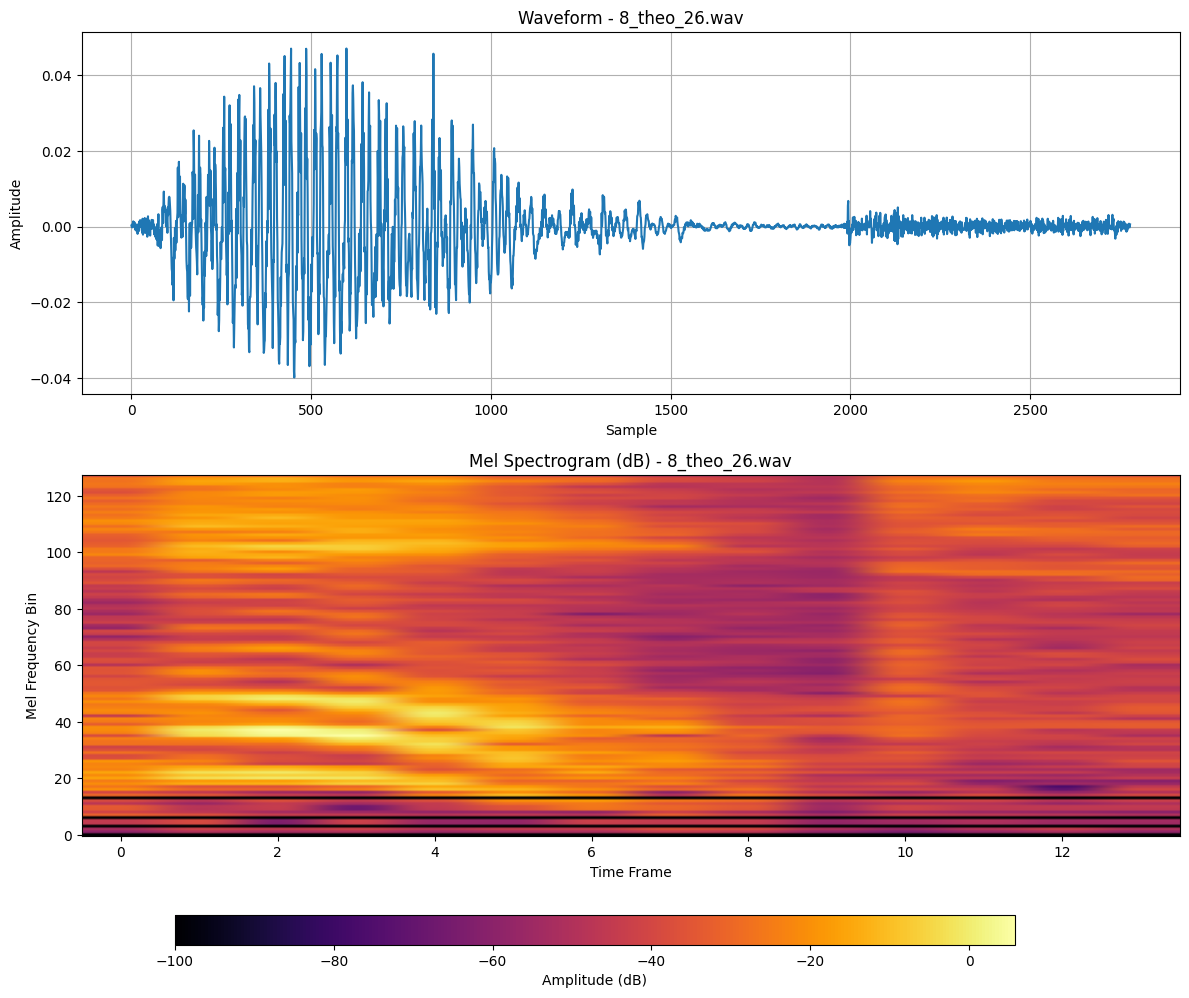
\includegraphics[width=0.9\textwidth]{WaveSpectro_1.png}
    \caption{Visualisation combinée: forme d'onde (haut) et spectrogramme Mel (bas) d'un fichier audio "8\_theo\_26.wav"}
    \label{fig:waveform_spec}
\end{figure}

Pour chaque fichier analysé, les informations suivantes ont été extraites:
\begin{itemize}
    \item Taux d'échantillonnage: 8000 Hz
    \item Forme de l'onde: 1 canal audio, durée variable (~2500-2800 échantillons)
    \item Forme du spectrogramme: 128 bandes de fréquences, ~13-14 fenêtres temporelles
    \item Durée moyenne: ~0.3-0.35 secondes
\end{itemize}

\begin{table}[h]
    \centering
    \renewcommand{\arraystretch}{1.2} % Espacement entre les lignes
    \begin{tabular}{>{\ttfamily}l l} 
        \toprule
        \textbf{Paramètre} & \textbf{Valeur} \\
        \midrule
        Fichier & 8\_theo\_26.wav \\
        Sample rate & 8000 Hz \\
        Forme de l'onde & [1, 2779] \\
        Forme du spectrogramme & [1, 128, 14] \\
        Durée de l'audio & 0.35 seconds \\
        \bottomrule
    \end{tabular}
\end{table}

\begin{figure}[H]
    \centering
    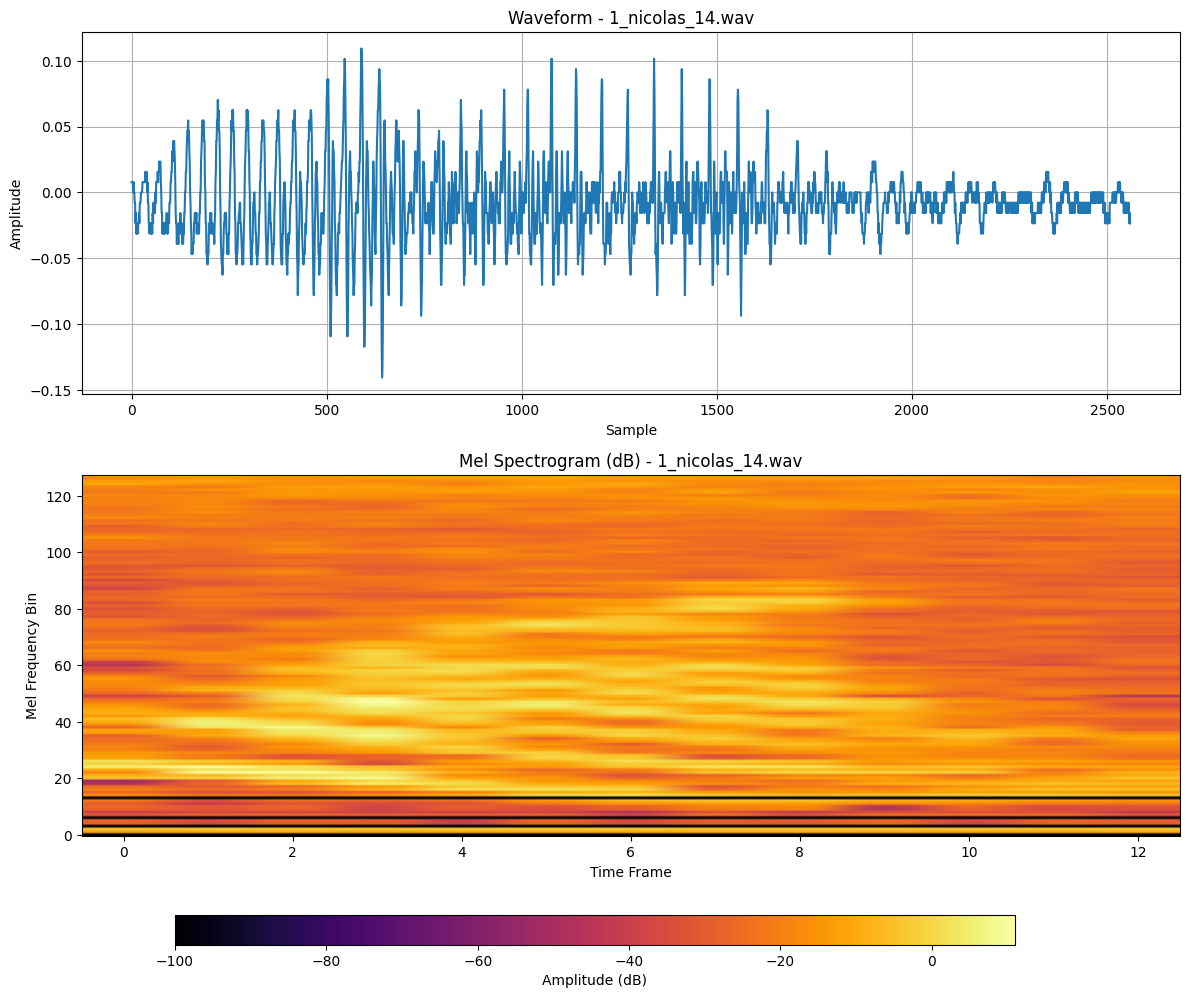
\includegraphics[width=0.9\textwidth]{WaveSpectro_2.png}
    \caption{Visualisation combinée: forme d'onde (haut) et spectrogramme Mel (bas) d'un fichier audio "1\_nicolas\_14.wav"}
    \label{fig:waveform_spec}
\end{figure}

\begin{table}[h]
    \centering
    \renewcommand{\arraystretch}{1.2} % Espacement entre les lignes
    \begin{tabular}{>{\ttfamily}l l} 
        \toprule
        \textbf{Paramètre} & \textbf{Valeur} \\
        \midrule
        Fichier & 1\_nicolas\_14.wav \\
        Sample rate & 8000 Hz \\
        Forme de l'onde & [1, 2560] \\
        Forme du spectrogramme & [1, 128, 13] \\
        Durée de l'audio & 0.32 seconds \\
        \bottomrule
    \end{tabular}
\end{table}



\section{Préparation des données d'entraînement et de test}
\label{sec:preparation}

\subsection{!!!!!!!! Séparation train/test !!!!!!!!}
\label{subsec:split}

Le script \texttt{SplitTrainTest\_original.py} a été utilisé pour diviser le jeu de données en deux sous-ensembles : 75\% des données pour l'entraînement et 25\% pour les tests, contrairement à la répartition 80/20 vue précédemment. Cette séparation est réalisée de manière aléatoire tout en garantissant une répartition équilibrée des classes. 

Pour cela, l'ensemble des données est préalablement mélangé afin d'assurer une représentation relativement équitable de chaque modalité cible dans les ensembles d'entraînement et de test.

\begin{lstlisting}
# Exécution du script de séparation
python SplitTrainTest_original.py
\end{lstlisting}

\subsection{Analyse de la répartition des données}
\label{subsec:analyse_repartition}

L'analyse des fichiers CSV générés confirme que:
\begin{itemize}
    \item Ensemble d'entraînement: 2250 échantillons (75\%)
    \item Ensemble de test: 750 échantillons (25\%)
    \item Les deux ensembles contiennent des enregistrements de 6 locuteurs différents
    \item La répartition des chiffres est parfaitement équilibrée dans le jeu complet, et relativement équilibrée dans les sous-ensembles de données générées aléatoirement. 
\end{itemize}

\begin{table}[H]
    \centering
    \caption{Répartition des classes dans les ensembles de test, et d'entraînement}
    \label{tab:repartition}
    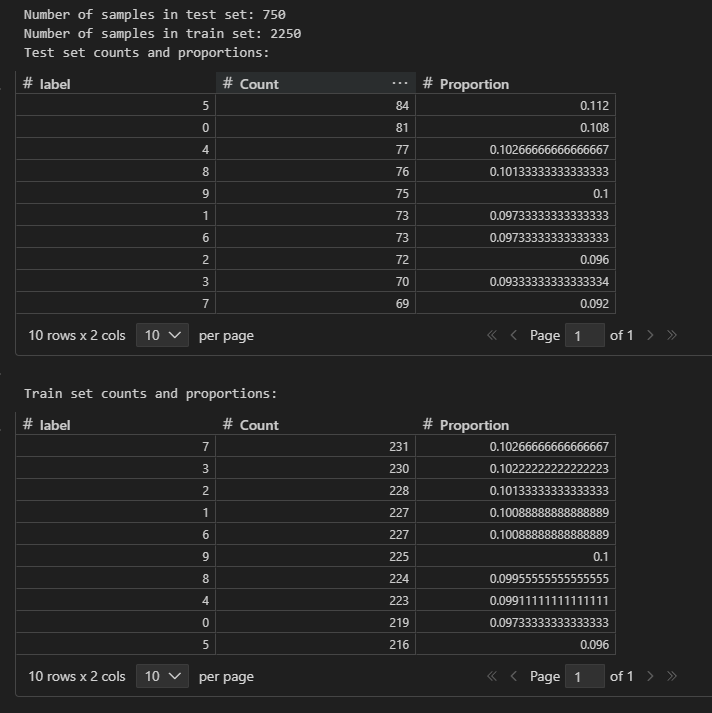
\includegraphics[width=0.9\textwidth]{Tables_LablesProps_Test_Train.png}
\end{table}


\section{Analyse du modèle de reconnaissance}
\label{sec:analyse_modele}

\subsection{Description du modèle}
\label{subsec:description_modele}

\subsubsection{Block 11}
Le block 11 définit une classe CNN (Convolutional Neural Network), contenant une initialisation et une méthode :
\begin{itemize}
    \item L'initialisation définit une séquence d'opérations comme l'algorithme ConvNet, utilisant des méthodes héritées de \texttt{nn.Module}. Elle définit l'architecture du réseau de neurones, ses couches :
    \begin{enumerate}
        \item Convolution 2D, avec 1 canal d'entrée, 10 de sortie et un noyau de taille $7 \times 7$ et un pas de 3. Cette couche produit 10 feature maps pour chaque donnée d'entrée, le filtre faisant cela est de taille $7 \times 7$ permettant de détecter des patterns dans les données.
        \item Fonction d'activation ReLU, appliquée à la 1\iere{} couche (introduit de la non-linéarité).
        \item Convolution 2D, avec 10 canaux d'entrée, 10 de sortie et un noyau de taille $5 \times 5$ et un pas de 2. La couche prend en entrée les 10 features maps de la couche précédente, le filtre appliqué aux feature maps est de taille $5 \times 5$, appliqué à chaque feature map il effectue des convolutions sur les données. Le pas et le kernel diminués permettent de diminuer la taille de la sortie de la 2\ieme{} couche comparée à la 1\iere{}.
        \item Fonction d'activation ReLU, appliquée à la 2\ieme{} couche.
        \item Aplatissement des données (couche de neurones) en un vecteur 1D.
        \item Application d'une fonction affine linéaire aux données, prend en entrée un vecteur de grande taille ($38 \times 19 \times 10$), et donne un vecteur de taille 10 en sortie.
    \end{enumerate}
    \item La méthode \texttt{forward} permet de passer des données dans le réseau défini précédemment. On passe une donnée X dans le réseau et on sort les logits, score brut (avant l'application de la fonction d'activation) pour chaque classe prédite.
\end{itemize}

\subsubsection{Block 12}
Le block 12 crée un modèle à partir de la classe CNN. Ce modèle est transféré sur un dispositif qui sera le GPU s'il y en a un, et le CPU sinon.

\subsubsection{Block 13}
Le block 13 initialise la fonction de perte d'entropie croisée de PyTorch. Elle permet de mesurer les écarts entre prédictions du modèle et vraies étiquettes des données, la Loss. Cela permet d'évaluer la performance du modèle créé. Plus la Loss est faible, plus le modèle est bon.

Ensuite, le block contient un optimiseur de modèle via un gradient. Il permet d'ajuster les poids du modèle pour minimiser la Loss. Les paramètres du gradient sont : un taux d'apprentissage à 0.001 (taille des mises à jour de poids), et un momentum de 0.9 (aide à converger plus rapidement).

\subsubsection{Block 14}
Ce block définit 2 fonctions :
\begin{itemize}
    \item La fonction \texttt{train}, utilise le modèle CNN prédéfini, l'optimiseur, la fonction permettant de calculer la Loss, et des données d'entrée.
    La fonction, pour des lots de données :
    \begin{enumerate}
        \item Charge les données (dans le format adapté au device (GPU ou CPU)) et les normalise,
        \item Utilise le modèle CNN en mode entraînement pour activer le calcul des gradients,
        \item Ensuite les opérations "Forward Pass" ont lieu : récupère les prédictions de labels faites par le modèle, calcule la loss,
        \item Met à jour les indicateurs globaux de la loss totale et du nombre de prédictions correctes,
        \item Enfin a lieu le "Backward Pass", on utilise la backpropagation via l'optimiseur gradient (reset du gradient, calculs des pertes pour les paramètres, mise à jour des paramètres du gradient),
        \item La fonction renvoie la perte moyenne et le score du modèle (précision).
    \end{enumerate}
    
    \item La fonction \texttt{test}, utilise le modèle CNN et la fonction de calcul de la Loss.
    La fonction, par lots :
    \begin{enumerate}
        \item Charge les données (dans le format adapté au device (GPU ou CPU)) et les normalise,
        \item Utilise le modèle CNN en mode évaluation sans activer le calcul des gradients,
        \item Ensuite on fait uniquement une opération "Forward Pass", on utilise le modèle et récupère les prédictions,
        \item Calcule la Loss de ce modèle et met à jour les indicateurs globaux,
        \item Enfin, la fonction renvoie la perte moyenne et le score du modèle (précision).
    \end{enumerate}
\end{itemize}

\subsubsection{Block 15}
Dans ce block, on utilise tous les éléments et fonctions définis précédemment. Pour 30 epochs, on entraîne et teste le modèle, en ajoutant tous les indicateurs de performance (loss et score de précision) à des listes pour les conserver.

\subsection{Architecture du modèle CNN}
\label{subsec:architecture}

Le modèle utilisé est un réseau de neurones convolutif (CNN) avec l'architecture suivante:

\begin{enumerate}
    \item \textbf{Première couche convolutive:}
    \begin{itemize}
        \item 1 canal d'entrée, 10 canaux de sortie
        \item Noyau de taille $7 \times 7$, et un pas de 3
        \item Détecte les motifs de base dans les spectrogrammes
    \end{itemize}
    
    \item \textbf{Fonction d'activation ReLU} après la première couche
    
    \item \textbf{Seconde couche convolutive:}
    \begin{itemize}
        \item 10 canaux d'entrée, 10 canaux de sortie
        \item Noyau de taille $5 \times 5$, pas de 2
        \item Traite les feature maps de la première couche
    \end{itemize}
    
    \item \textbf{Fonction d'activation ReLU} après la seconde couche
    
    \item \textbf{Aplatissement} des données en vecteur 1D
    
    \item \textbf{Couche fully connected} qui réduit le vecteur aplati à 10 sorties, une pour chaque chiffre
\end{enumerate}

\begin{figure}[H]
    \centering
    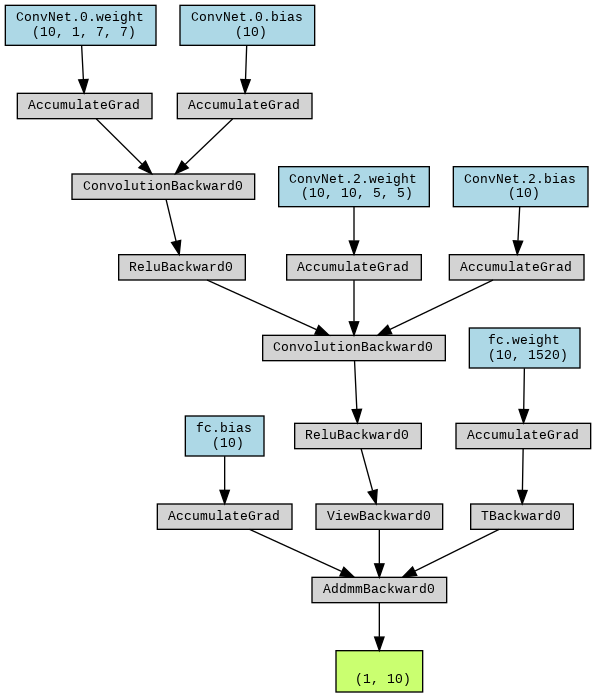
\includegraphics[width=0.9\textwidth]{Schema_CNN_Audio.png}
    \caption{Architecture du réseau de neurones convolutif utilisé pour la reconnaissance des chiffres prononcés}
    \label{fig:cnn_archi}
\end{figure}

\subsection{Fonction de perte et optimisation}
\label{subsec:loss_optim}

Le modèle utilise:
\begin{itemize}
    \item \textbf{Fonction de perte:} Cross-Entropy Loss, adaptée pour les problèmes de classification
    \item \textbf{Optimiseur:} Stochastic Gradient Descent (SGD) avec:
    \begin{itemize}
        \item Taux d'apprentissage: 0.001
        \item Momentum: 0.9 pour accélérer la convergence
    \end{itemize}
\end{itemize}

\subsection{Processus d'entraînement et d'évaluation}
\label{subsec:training}

Le processus comprend deux fonctions principales:
\begin{itemize}
    \item \textbf{Fonction train:}
    \begin{itemize}
        \item Active le mode entraînement du modèle
        \item Normalise les données d'entrée
        \item Effectue une passe avant pour obtenir les prédictions
        \item Calcule la perte et met à jour les indicateurs
        \item Effectue une passe arrière (backpropagation) pour ajuster les poids
    \end{itemize}
    
    \item \textbf{Fonction test:}
    \begin{itemize}
        \item Active le mode évaluation du modèle (sans calcul de gradients)
        \item Normalise les données d'entrée
        \item Effectue uniquement une passe avant
        \item Calcule la perte et les métriques de performance
    \end{itemize}
\end{itemize}

L'entraînement se déroule sur 30 époques, avec un suivi de la perte et de la précision pour les ensembles d'entraînement et de test.

\subsection{Analyse des performances}
\label{subsec:performances}

Les courbes d'apprentissage montrent :

\begin{figure}[H]
    \centering
    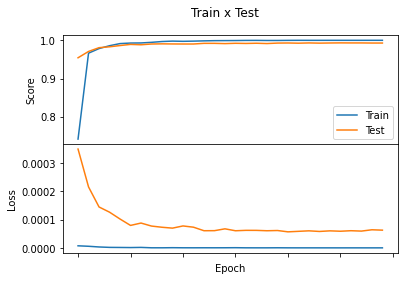
\includegraphics[width=0.8\textwidth]{learning_curves.png}
    \caption{Évolution de la précision et de la perte durant l'entraînement}
    \label{fig:curves}
\end{figure}

\begin{itemize}
    \item \textbf{Précision (accuracy) :}
    \begin{itemize}
        \item Ensemble d'entraînement : La précision atteint rapidement une valeur proche de 100\%, ce qui indique une excellente performance du modèle sur cet ensemble, un apprentissage quasi parfait sur l'ensemble d'entraînement..
        \item Ensemble de test : La précision se stabilise à une valeur élevée mais légèrement inférieure à celle de l'entraînement, ce qui reflète une généralisation correcte, bien que légèrement moins performante que sur l'ensemble d'entraînement.
    \end{itemize}
    
    \item \textbf{Perte (loss) :}
    \begin{itemize}
        \item Ensemble d'entraînement : La perte diminue rapidement et se stabilise à une valeur très basse, ce qui indique que le modèle s'adapte bien aux données d'entraînement.
        \item Ensemble de test : La perte continue de diminuer, mais elle reste plus élevée que celle observée pour l'entraînement, ce qui suggère un léger écart entre les performances sur les ensembles d'entraînement et de test. 
    \end{itemize}
    
    \item \textbf{Interprétation :} L'écart entre les performances d'entraînement et de test suggère un léger surapprentissage (overfitting). Cependant, étant donné que les résultats sur l'ensemble de test restent bons, cela montre que le modèle généralise correctement, bien que des ajustements pour limiter l'overfitting pourraient être nécessaires.
\end{itemize}

\subsection{Quel modèle ?}
\label{subsec:quel_modele}

Les blocs 11 à 15 décrivent un modèle de réseau de neurones convolutif (CNN) pour la classification multimodale d'images et de spectrogrammes audio. Le modèle est entraîné à l'aide de PyTorch, avec des fonctions de perte et des optimisateurs pour ajuster les poids du réseau. Le processus d'entraînement et de test est itératif, avec des évaluations de la performance à chaque époque pour suivre la précision et la perte du modèle.

\section{Proposition d'un système multimodal}
\label{sec:multimodal}

\subsection{Objectif}
\label{subsec:objectif_multi}

L'objectif est de créer un système multimodal qui combine:
\begin{itemize}
    \item La reconnaissance visuelle des chiffres écrits (MNIST)
    \item La reconnaissance acoustique des chiffres prononcés (AudioMNIST)
\end{itemize}

Cette fusion vise à améliorer la performance globale du système en tirant parti de la complémentarité des deux modalités.

\subsection{Méthodologie proposée}
\label{subsec:methodologie}

\subsubsection{Préparation des données}
\label{subsubsec:prep_multi}

\paragraph{MNIST (Images)}
\begin{itemize}
    \item Chargement via torchvision
    \item Normalisation des images
    \item Division en ensembles d'entraînement et de test
\end{itemize}

\paragraph{AudioMNIST (Audio)}
\begin{itemize}
    \item Uniformisation de la durée des signaux
    \item Conversion en MelSpectrogrammes
    \item Application d'une transformation logarithmique (pour plus de robustesse)
    \item Division en ensembles d'entraînement et de test
\end{itemize}

\paragraph{Extraction des Caractéristiques (features)}
\begin{itemize}
    \item Pour MNIST, les pixels des images constituent les features.
    \item Pour AudioMNIST, extraire des caractéristiques à partir des MelSpectrograms.
\end{itemize}

\subsubsection{Conception du modèle}
\label{subsubsec:conception}

\paragraph{Modèles indépendants}
\begin{itemize}
    \item \textbf{Modèle image:} CNN pour MNIST
    \item \textbf{Modèle audio:} CNN ou RNN pour AudioMNIST
\end{itemize}

\paragraph{Stratégies de fusion}

\begin{figure}[H]
    \centering
    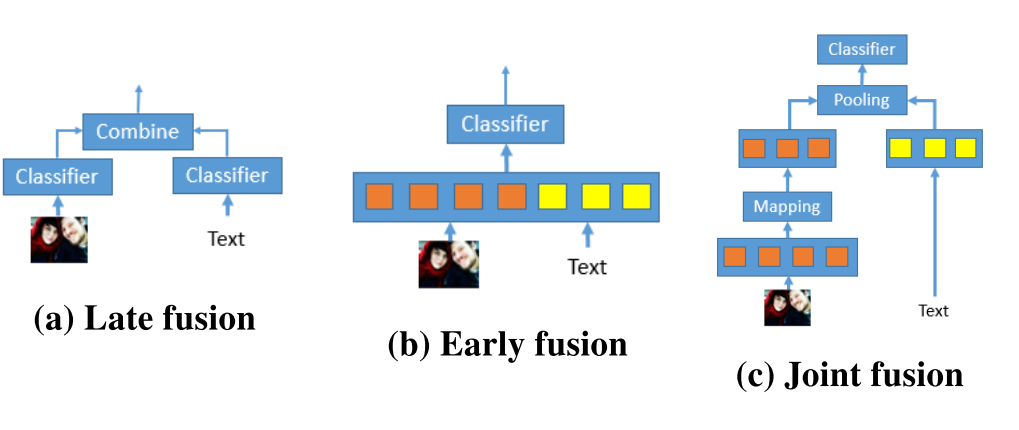
\includegraphics[width=0.9\textwidth]{fusion_strategies.png}
    \caption{Illustration des différentes stratégies de fusion multimodale}
    \label{fig:fusion}
\end{figure}

\begin{itemize}
    \item \textbf{Fusion précoce (Early fusion) (b):}
    \begin{itemize}
        \item Concaténation des caractéristiques brutes
        \item Permet d'apprendre des corrélations à bas niveau
        \item Nécessite d'harmoniser les dimensions des modalités
    \end{itemize}
    
    \item \textbf{Fusion intermédiaire (Joint fusion) (c):}
    \begin{itemize}
        \item Extraction séparée des caractéristiques pour chaque modalité
        \item Fusion des représentations obtenues
        \item Options : concaténation, couche d'attention
    \end{itemize}
    
    \item \textbf{Fusion tardive (Late fusion) (a):}
    \begin{itemize}
        \item Chaque modalité est traitée indépendamment par un classificateur
        \item Les prédictions finales sont combinées pour obtenir une décision finale
        \item Méthodes : moyenne pondérée, vote majoritaire
        \item Avantage : robuste en cas de défaillance d’une modalité
    \end{itemize}    
\end{itemize}

\paragraph{Architecture proposée}
\begin{itemize}
    \item Encodeurs spécifiques à chaque modalité  (CNN pour images, CNN/RNN pour audio)
    \item Mécanisme d'attention pour pondérer l'importance des modalités
    \item Couches fully connected finales pour la classification
\end{itemize}

\subsubsection{Entraînement et évaluation}
\label{subsubsec:train_eval}

\begin{itemize}
    \item Entraînement des modèles individuels
    \item Entraînement du modèle fusionné
    \item Comparaison des performances:
    \begin{itemize}
        \item Modèle visuel seul
        \item Modèle audio seul
        \item Modèle multimodal
    \end{itemize}
    \item Analyse des cas où une modalité est plus fiable que l'autre
\end{itemize}

\subsubsection{Optimisation}
\label{subsubsec:optimisation}

\begin{itemize}
    \item Expérimentation avec différentes architectures
    \item Ajustement des hyperparamètres
    \item Augmentation des données
    \item Raffinement de la stratégie de fusion
\end{itemize}

\section{Conclusion}
\label{sec:conclusion}

Ce TP a permis d'explorer en profondeur les techniques de traitement et de reconnaissance des signaux audio, en utilisant le jeu de données AudioMNIST. Nous avons:
\begin{itemize}
    \item Analysé et visualisé des signaux audio et leurs représentations fréquentielles
    \item Étudié l'architecture d'un réseau de neurones convolutif pour la reconnaissance de chiffres prononcés
    \item Analysé le processus d'entraînement et les performances du modèle
    \item Proposé une approche multimodale combinant reconnaissance visuelle et auditive
\end{itemize}

La proposition d'un système multimodal ouvre des perspectives intéressantes pour améliorer la robustesse et la précision de la reconnaissance des chiffres. Cette approche pourrait être étendue à d'autres applications nécessitant l'intégration de plusieurs modalités perceptives.

\begin{figure}[H]
    \centering
    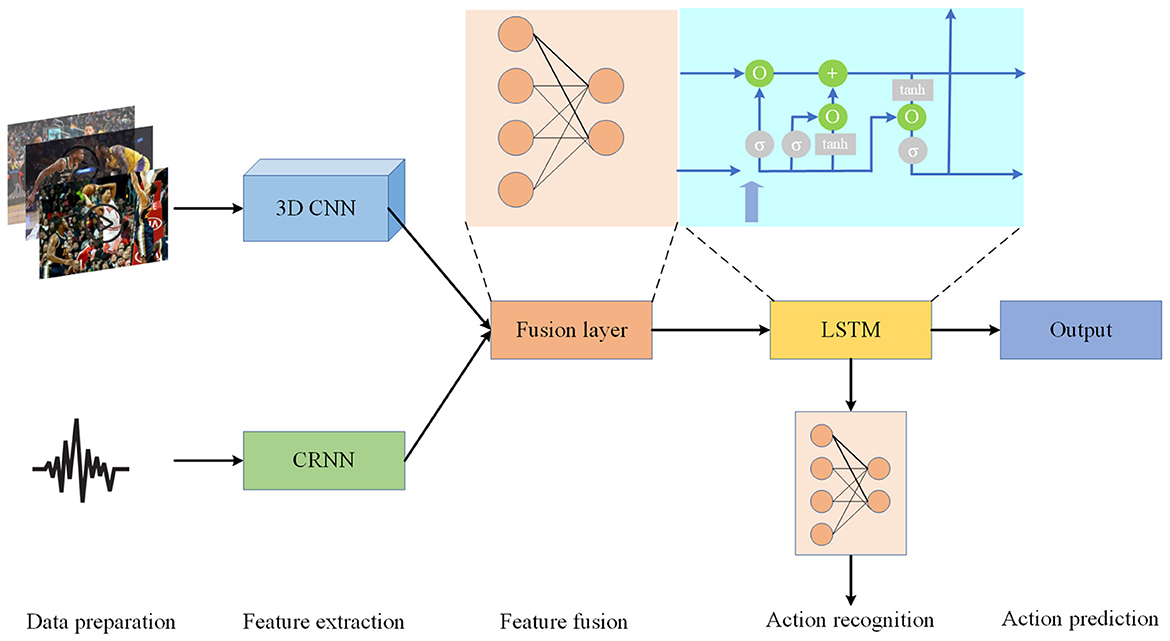
\includegraphics[width=0.9\textwidth]{multimodal_system.jpg}
    \caption{Architecture générale du système multimodal proposé}
    \label{fig:system}
\end{figure}

\section{Références}
\label{sec:references}

\begin{thebibliography}{9}
    \bibitem{kaggle} Jokekling, "PyTorch Study Audio", Kaggle, \url{https://www.kaggle.com/code/jokekling/pytorch-study-audio}
    \bibitem{audiomnist} Becker, S., Ackermann, M., Lapuschkin, S., Müller, K. R., & Samek, W. (2018). "Interpreting and explaining deep neural networks for classification of audio signals." arXiv preprint arXiv:1807.03418.
    \bibitem{mel} Stevens, S. S., Volkmann, J., & Newman, E. B. (1937). "A scale for the measurement of the psychological magnitude pitch." The Journal of the Acoustical Society of America, 8(3), 185-190.
    \bibitem{pytorch} Paszke, A., Gross, S., Massa, F., Lerer, A., Bradbury, J., Chanan, G., ... & Chintala, S. (2019). "PyTorch: An imperative style, high-performance deep learning library." In Advances in Neural Information Processing Systems (pp. 8026-8037).
\end{thebibliography}

\appendix
\section{Code complet}
\label{app:code}

\begin{lstlisting}
# Code pour la visualisation des spectrogrammes
import torch
import torchaudio
from matplotlib import pyplot as plt

# Définition des transformations
ToSpectrogram = torchaudio.transforms.MelSpectrogram()
ToDB = torchaudio.transforms.AmplitudeToDB()

# Chargement et visualisation d'un fichier audio
file_path = os.path.join(directory, file)
waveform, sample_rate = torchaudio.load(file_path)
spectrogram = ToSpectrogram(waveform)
spec_db = ToDB(spectrogram)

# Création de la figure
fig, axs = plt.subplots(2, 1, figsize=(12, 10))
# Plot waveform
axs[0].plot(waveform.t().numpy())
# Plot spectrogram
axs[1].imshow(spec_db[0].numpy(), origin="lower", aspect="auto", cmap="inferno")
\end{lstlisting}

\end{document}